\documentclass[12pt,a4paper]{amsart}
% ukazi za delo s slovenscino -- izberi kodiranje, ki ti ustreza
\usepackage[slovene]{babel}
%\usepackage[cp1250]{inputenc}
%\usepackage[T1]{fontenc}
\usepackage[utf8]{inputenc}
\usepackage{amsmath,amssymb,amsfonts}
\usepackage{url}
%\usepackage[normalem]{ulem}
\usepackage[dvipsnames,usenames]{color}
\usepackage{graphicx}

\usepackage[table,xcdraw]{xcolor}

\usepackage{listings}
\usepackage{color}
 
\definecolor{codegreen}{rgb}{0,0.6,0}
\definecolor{codegray}{rgb}{0.5,0.5,0.5}
\definecolor{codepurple}{rgb}{0.58,0,0.82}
\definecolor{backcolour}{rgb}{0.95,0.95,0.92}

\lstdefinestyle{mystyle}{
    backgroundcolor=\color{backcolour},   
    commentstyle=\color{codegreen},
    keywordstyle=\color{magenta},
    numberstyle=\tiny\color{codegray},
    stringstyle=\color{codepurple},
    basicstyle=\footnotesize,
    breakatwhitespace=false,         
    breaklines=true,                 
    captionpos=b,                    
    keepspaces=true,                 
    numbers=left,                    
    numbersep=5pt,                  
    showspaces=false,                
    showstringspaces=false,
    showtabs=false,                  
    tabsize=2
}
 
\lstset{style=mystyle}

% ne spreminjaj podatkov, ki vplivajo na obliko strani
\textwidth 15cm
\textheight 24cm
\oddsidemargin.5cm
\evensidemargin.5cm
\topmargin-5mm
\addtolength{\footskip}{10pt}
\pagestyle{plain}
\overfullrule=15pt % oznaci predlogo vrstico


% ukazi za matematicna okolja
\theoremstyle{definition} % tekst napisan pokoncno
\newtheorem{definicija}{Definicija}[section]
\newtheorem{primer}[definicija]{Primer}
\newtheorem{opomba}[definicija]{Opomba}

\renewcommand\endprimer{\hfill$\diamondsuit$}


\theoremstyle{plain} % tekst napisan posevno
\newtheorem{lema}[definicija]{Lema}
\newtheorem{izrek}[definicija]{Izrek}
\newtheorem{trditev}[definicija]{Trditev}
\newtheorem{posledica}[definicija]{Posledica}


% za stevilske mnozice uporabi naslednje simbole
\newcommand{\R}{\mathbb R}
\newcommand{\N}{\mathbb N}
\newcommand{\Z}{\mathbb Z}
\newcommand{\C}{\mathbb C}
\newcommand{\Q}{\mathbb Q}


% ukaz za slovarsko geslo
\newlength{\odstavek}
\setlength{\odstavek}{\parindent}
\newcommand{\geslo}[2]{\noindent\textbf{#1}\hspace*{3mm}\hangindent=\parindent\hangafter=1 #2}


% naslednje ukaze ustrezno popravi
\newcommand{\program}{Finančna matematika} % ime studijskega programa
\newcommand{\imeavtorja}{Katarina Brilej, Sara Kovačič} % ime avtorja
\newcommand{\imementorja}{prof.~dr. Riste Škrekovski} % akademski naziv in ime mentorja
\newcommand{\naslovdela}{Uporaba metahevristike GRASP na problemu potujočega trgovca}
\newcommand{\letnica}{2019} %letnica 


% vstavi svoje definicije ...




\begin{document}

% od tod do povzetka ne spreminjaj nicesar
\thispagestyle{empty}
\noindent{\large
UNIVERZA V LJUBLJANI\\[1mm]
FAKULTETA ZA MATEMATIKO IN FIZIKO\\[5mm]
\program\ -- 1.~stopnja}
\vfill

\begin{center}{\large
\imeavtorja\\[2mm]
{\bf \naslovdela}\\[10mm]
Projekt OR pri predmetu Finančni praktikum\\[1cm]
Mentor: \imementorja}
\end{center}
\vfill

\noindent{\large
Ljubljana, \letnica}
\pagebreak

\thispagestyle{empty}
\tableofcontents
\pagebreak


% tu se zacne besedilo seminarja
\section{Uvod}

Metahevristika je algoritemski način reševanja kombinatoričnega optimizacijskega problema, pri katerem na začetku izberemo množico kandidatov za rešitev, in jo iterativno izboljšujemo (glede na neko vnaprej izbrano funkcijo zaželenosti), ter po dovolj korakih vrnemo najboljši element iz te množice. Metahevristike torej vrnejo približne rešitve, a veliko hitreje kot eksaktni postopki. V projektu bova na problem potujočega trgovca implementirali metahevristiko GRASP (\textit{greedy randomized adaptive search procedure}). Problem potujočega trgovca bova rešili tudi kot celoštevilski linearni program in primerjali rešitve. Generirali bova nekaj zanimivih grafov in na njih preizkusili algoritem. Rezultate bova primerjail tudi z rezultati iz spleta in rezultati skupine 7, ki bo na problem potujočega trgovca implementirala genetski algoritem. 


\section{Problem potujočega trgovca} 

Problem potujočega trgovca (”travelling salesman problem”/TSP) se glasi:


\begin{itemize}
\item {\bf Formulacija v vsakdanjem jeziku:} danih je $n$ mest in razdalja med poljubnim parom mest (od mesta do mesta lahko potujemo po zgolj eni poti). Najdi najkrajšo (najcenejšo) pot, ki se začne in konča v istem mestu ter obišče vsako mesto natanko enkrat.
\item{\bf Formulacija v matematičnem jeziku}: v (neusmerjenem enostavnem) polnem grafu $K_n$ z uteženimi povezavami (pozitivne vrednosti) najdi najkrajši cikel, ki vsebuje vsa vozlišča. Ciklom, ki vsebujejo vsa vozlišča grafa, pravimo Hamiltonovi cikli.

\end{itemize}


\section{Grasp} 

GRASP (\textit{greedy randomized adaptive search procedure}) je metahevristika, ki sestoji iz dveh faz: \textit{greedy randomized construction} in \textit{local search}.
V prvi fazi na pameten način (odvisno od problema) izberemo izmed vseh možnih rešitev CL (candidate list) množico začetnih približkov RCL (restricted candidates list). 
To storimo deloma deterministično in deloma stohastično, da zagotovimo, da so začetni približki obetavni, a dovolj razpršeni po celotni množici CL, da bo druga faza pregledala čimvečji del CL. 
V drugi fazi za vsako izmed teh rešitev $ s \in  RCL $ pregledamo elemente $s' \in CL$ v njeni okolici (kaj je okolica je od problema in načina reševanja odvisno). Če najdemo boljšo rešitev $s'$, 
jo dodamo v RCL ter $s$ odstranimo. To ponavljamo dokler zaustavitveni pogoj (npr. št. iteracij, zahtevana natančnost) ni izpolnjen.

\subsection{Greedy randomized construction} 

Kot smo "ze omenili je GRASP sestavljen iz dveh delov. Najprej bomo predstavili tako imenovan greedy randomized construction.
Tu parameter alpha predstavlja mo"c mno"zice za"cetnih pribli"zkov (RCL), v na"sem primeru torej dol"zino seznama RCL.
Za vhodni podatek imamo tudi inciden"cno matriko cen povezav velikosti nxn. g je simetri"cna matrika, z ni"clami po diagonali.
Na za"cetku jo s pomo"cjo funkcije slovar\_cen spremenimo v slovar, sestavljen iz elementov, ki jo imajo za klju"c povezavo oblike ($x_{i}$, $x_{j}$), za vrednost pa ceno/razdaljo, ki ji pripada. Vsak za"cetni pribli"zek $t = (l,1,v_{2}, \dots,v_{n})$ iz RCL konstruiramo tako, da dolo"cimo $v_{1} := 1$ nato iteraticno za$ i = 2, \dots,n$ za $v{i}$ izberemo naklju"cno med p \% najbli"zjih vozli"s"c do $v{i-1}$, ki "se niso v  $t$. Na koncu "se izra"cunamo dol"zino poti s prej definirano funkcijo dolzina\_poti in jo postavimo na ni"cto mesto. Take cikle $t$ konstruiramo toliko 2casa, da RCL napolnimo. "Ce delamo z matrikami velikosti manj kot 5, moramo nastaviti tudi parameter deles, saj mora vrednost n // delez presegati "stevilo 1.  


\begin{lstlisting}[language=Python]
def greedy_construction(g, alpha, delez = 5):
    RCL = [0] * alpha
    slovar = slovar_cen(g)
    n = len(g)
    p = n // delez
    for j in range(0, alpha):
        t = [0] * (n+1)
        t[1] = 1
        mesta = [h for h in range(2,n+1)]
        for i in range(2,n+1):
            povezave = [(t[i-1],m) for m in mesta]
            cene = { key:value for key, value in slovar.items() if key in povezave }
            urejene_povezave = sorted(cene, key=cene.__getitem__)
            (_,vi) = random.choice(urejene_povezave[:p])
            t[i] = vi
            mesta.remove(vi)
        t[0] = dolzina_poti(g,t)
        RCL[j] = t
    return RCL
\end{lstlisting}

\subsection{Local search} 

V tem delu se bomo posvetili drugemu delu algoritma imenovanemu local search. Obravnavali bomo dve metodi 2opt in 3opt. Funkcija local\_search zato poleg matrike g, parametra alpha in "stevila iteracij sprejme "se parameter metodo. 
Na za"cetku definiramo RCL, ki predstavlja za"cetni seznam pribli"zkov. Te nato uredimo po dol"zini, primerjamo jih po prvem elementu, ki predstavlja dol"zino poti. Nato naklju"cno izberemo t iz RCL, toda z linerano padajo"co verjetnostjo. Najverjetneje izbereme cikel na vrhu RCL , torej najkraj"si. Ko imamo izbran t se na podlagi parametra metoda odlo"cimo za 2opt ali pa 3opt. Obe metodi poizku"sata pribli"zek izbolj"sati, "ce jima uspe, vrneta novi\_t. Neodvisno od metode nato v primeru, da je izbolj"sava uspela v RCL dodamo izbolj"san pribli"zek in starega odstranimo. Kasneje si bomo ogledali "se kako posamezna metoda deluje. Ponavljamo tolikokrat kot je predpisano, to nam dolo"ca iter. 


\begin{lstlisting}[language=Python]
def local_search(g,k,iter,metoda):
    RCL = greedy_construction(g,k)
    n = len(g)
    slovar = slovar_cen(g)
    #urejen seznam zacetnih priblizkov
    RCL.sort(key=lambda x: x[0])
    stevec = 0
    while stevec < iter:
        utezi = [i * 2/((k+1)*k) for i in range(k,0,-1)]
        indeks = np.random.choice(len(RCL), size = 1, p = utezi)
        t = RCL[indeks[0]]
        if metoda == "dva_opt":
            novi_t = dva_opt(n,t,g)
        elif metoda == "tri_opt":
            novi_t = tri_opt(n,t,g)      
        if novi_t:
            RCL.append(novi_t)
            RCL.remove(t)   
        stevec += 1
        RCL.sort(key=lambda x: x[0])
    RCL.sort(key=lambda x: x[0])
    return RCL[0]
\end{lstlisting}

"Ce si zdaj ogledamo "se kako delujeta posamezni metodi. Za"cnimo s preprostej"so, 2opt. 
Ko naklju"cno izberemo cikel t, ga "zelimo izbolj"sati. Kraj"si cikel i"s"cemo v okolici, ki je definirana kot monožica vseh ciklov t' iz CL, 
ki jih dobimo iz t tako, da mu zamenjamo dve vozišči, torej naključno zamenjamo dve vozlišči t. Namesto, da bi shranjevali vse mo"zne  t' in na koncu preverili, "ce je najkraj"si kraj"si od trenutnega t, je bolj u"cinkovito, "ce sproti preverjamo, "ce posamezna menjava prinese izbolj"savo. Na za"cetku zato definiramo spremenljivko razlika, ta meri, "ce je dana menjava bolj"sa. Nato moramo v zanki lo"citi dva primera, saj v primeru, da je j = n, razdremo povezavo s prvim elementom. Nato izra"cunamo change, "ce je ta manj"si od trenutne razlike, jo posodobimo, saj smo dobili kraj"si cikel. Shranimo si tudi optimalni i in j, da bomo na koncu vedeli s katero menjavo smo dosegli najkraj"si cikel. "Ce smo uspeli izbolj"sati t, bo razlika negativna in dobili bomo novi\_t. Tega konstruiramo tako, da na starem t izvedemo menjavo dolo"ceno z optimalnim i in j. Namesto, da znova ra"cunamo celotno dol"zino cikla, samo pri"stejemo razliko, ki je nagativna. 

\begin{lstlisting}[language=Python]
def dva_opt(n,t,g):
    slovar = slovar_cen(g)
    razlika = 0
    for i in range(2,n):
        for j in range(i+1,n+1):
            if j != n:
                change = slovar[(t[i-1],t[j])] + slovar[(t[i],t[j+1])] - slovar[(t[i-1],t[i])] - slovar[(t[j],t[j+1])]
            else:
                change = slovar[(t[i-1],t[j])] + slovar[(t[i],t[1])] - slovar[(t[i-1],t[i])] - slovar[(t[j],t[1])]               
            if change < razlika:
                razlika = change
                opt_i =  i
                opt_j = j
    if razlika < 0:
        novi_t = [t[m] for m in range(0,n+1)]
        novi_t[opt_i:opt_j+1] = novi_t[opt_i:opt_j+1][::-1]
        novi_t[0] = t[0] + razlika        
        return novi_t
    else:
        return None
\end{lstlisting}

3opt je nekoliko bolj dodelana razli"cica local searcha, zamenjamo namre"c kar tri vozli"s"ca. Tako kot 2opt sprejme velikost matrike, 
matriko in cikel t. Zaradi peglednosti na za"cetku definiramo spremenljivke X1, X2, Y1, Y2, Z1, Z2. Sedaj imamo 7 mo"znih menjav. Tri od teh so 2opt, "stiri pa 3opt. Za vsako od mo"znih menjav nato izra"cunamo razliko. Ker pri 3opt menjavah odstranimo enake povezave, lahko to shranimo pod spremenljivko odstej. Ko izra"cunamo vse razlike, poi"s"cemo minimum, s tem ko si zabele"zimo, pri katerem indeksu je bila minimalna razlika dose"zena, bomo kasneje vedeli katero menjavo izvesti, saj so te urejene po vrsti v seznamu spremembe. "Ce je change manj"sa od trenutne razlike, pomeni, da lahko t izbolj"samo. Posodobimo razliko, indeks in si zabele"zimo optimalne i,j in k, ki jih bomo potem potrebovali, da izvedemo ustrezno menjavo. Torej "ce je na koncu razlika manj"sa kot 0 lahko zgradimo novi\_t. Ta je odvisen od vrste menjave, ki jo moramo izvr"siti, ta pa je dolo"cena z indeksom in optimalnimi i,j in k. Tako kot pri 2opt tudi tukaj novo dol"zino cikla izra"cunamo tako, da pri"stejemo razliko. 

\begin{lstlisting}[language=Python]
def tri_opt(n, t, g):
    slovar = slovar_cen(g)
    razlika = 0    
    for i in range(2,n-1):
        for j in range(i+1,n):
            for k in range(j+1,n+1):
                X1, X2, Y1, Y2, Z1, Z2 = t[i-1], t[i], t[j-1], t[j], t[k-1], t[k]
# 2 opt moves
                change1 = slovar[(X1,Z1)] + slovar[(X2,Z2)] -  slovar[(X1,X2)] - slovar[(Z1,Z2)]
                change2 = slovar[(Y1, Z1)] + slovar[(Y2, Z2)] -  slovar[(Y1, Y2)] - slovar[(Z1, Z2)] 
                change3 = slovar[(X1, Y1)] + slovar[(X2, Y2)] -  slovar[(X1, X2)] - slovar[(Y1, Y2)]
# 3 opt moves
                odstej = slovar[(X1, X2)] + slovar[(Y1, Y2)] + slovar[(Z1, Z2)]
# v vseh treh primerih odstranimo enake povezave
                change4 = slovar[(X1, Y1)] + slovar[(X2, Z1)] + slovar[(Y2, Z2)] -  odstej
                change5 = slovar[(X1, Z1)] + slovar[(Y2, X2)] + slovar[(Y1, Z2)] -  odstej
                change6 = slovar[(X1, Y2)] + slovar[(Z1, Y1)] + slovar[(X2, Z2)] -  odstej
                change7 = slovar[(X1, Y2)] + slovar[(Z1, X2)] + slovar[(Y1, Z2)] -  odstej
# izracunamo najmanjso vrednost razlike
                spremembe = [change1,change2, change3, change4, change5,change6,change7]
                change = min(spremembe)
                ind = np.argmin(spremembe) + 1
                if change < razlika:
                    razlika = change
                    indeks = ind
                    opt_i =  i
                    opt_j = j
                    opt_k = k
    if razlika < 0:
        novi_t = menjava(indeks,n,t,opt_i,opt_j,opt_k)
        novi_t[0] = t[0] + razlika
        return novi_t
    else:
        return None
\end{lstlisting}

V naslednji funkciji so opisane menjave, ki jih moramo narediti na trenutnem ciklu t, odvisne pa so od indeksa. 

\begin{lstlisting}[language=Python]
def menjava(indeks,n,t,opt_i,opt_j,opt_k):   
    novi_t = [t[m] for m in range(0,n+1)]
    if indeks == 1:
        novi_t[opt_i:opt_k] = novi_t[opt_i:opt_k][::-1]
    if indeks == 2:
        novi_t[opt_j:opt_k] = novi_t[opt_j:opt_k][::-1]
    if indeks == 3:
        novi_t[opt_i:opt_j] = novi_t[opt_i:opt_j][::-1]      
    if indeks == 4:
        novi_t[opt_i:opt_j] = novi_t[opt_i:opt_j][::-1]
        novi_t[opt_j:opt_k] = novi_t[opt_j:opt_k][::-1]      
    if indeks == 5:
        tmp = novi_t[opt_j:opt_k][::-1] + novi_t[opt_i:opt_j]
        novi_t[opt_i:opt_k] = tmp        
    if indeks == 6:
        tmp = novi_t[opt_j:opt_k] + novi_t[opt_i:opt_j][::-1]
        novi_t[opt_i:opt_k] = tmp      
    if indeks == 7:
        tmp = novi_t[opt_j:opt_k] + novi_t[opt_i:opt_j]
        novi_t[opt_i:opt_k] = tmp
    return novi_t
\end{lstlisting}

\section{Celoštevilski linearni program} 

Problem potujočega trgovca lahko predstavimo kot \textit{celoštevilski linearni program}.
Označimo mesta s števili $1, \ldots, n$. Strošek (ali razdalja) potovanja iz mesta $i$ v mesto $j$ je $c_{i,j}$, ( $ 1\leq i, j\leq n$). Minimiziramo strošek potovanja. Definiramo:

$$ X_{i,j} := \left\{ \begin{array}{ll}
1 ~; & \textrm{potnik gre iz mesta $i$ v mesto $j$}, \\
0 ~; & \textrm{sicer},
\end{array} \right. $$

\hfill \break

$y_{i}$ \ldots katero po vrsti obiščemo mesto $i$

\begin{equation*}
\begin{aligned}
& {\text{min}}
& & \sum_{i=1}^{n} \sum_{j=1}^{n}  x_{i,j} \cdot c_{i,j} \\
& \text{p. p.}
& &\sum_{i=1}^{n} x_{i,j} = 1, \text{ za vsak $j$ }\\
&&&\sum_{j=1}^{n} x_{i,j} = 1, \text{ za vsak $i$ }\\
&&&  x_{i,j} \in \{0,1\}, \text{ za vsak $i$ in vsak $j$ }\\
&&& y_{i} \in \{1, \ldots, n\}; \text{za vsak $i$}\\
&&& y_{i} + 1 - n + n \cdot x_{i,j} \leq y_{j}; \text{za vsak $i$ in vsak $j>1$}
\end{aligned}
\end{equation*}
\\
Problem potujočega trgovca se da v Pythonu elegantno zapisati kot celoštevilski linearni program s pomočjo knjižnice PuLP. PuLP za reševanje problema izbere enega od vgrajenih algoritmov. V našem primeru je PuLP za reševanje izbral PULP\_CBC\_CMD. S pomočjo knjižnice PuLP sva napisali funckijo, ki sprejme matriko cen povezav, izpiše minimalno ceno potovanja in vrne urejen seznam obiskanih mest.

\begin{lstlisting}[language=Python]
from pulp import *
def tsp_as_ilp(g):
    razdalje = slovar_cen_ilp(g)   # slovar razdalj 
    mesta = [x+1 for x in range(len(g))]  # seznam mest (od 1 do n)
    prob = LpProblem("salesman", LpMinimize) # definiramo problem
    x = LpVariable.dicts('x', razdalje, 0,1, LpBinary) 
    cena = lpSum([x[(i,j)]*razdalje[(i,j)] for (i,j) in razdalje]) 
    prob += cena
    for k in mesta:  # pri pogojih:
        prob += lpSum([ x[(i,k)] for i in mesta if (i,k) in x]) == 1  
        prob += lpSum([ x[(k,i)] for i in mesta if (k,i) in x]) == 1  
    u = LpVariable.dicts('u', mesta, 0, len(mesta)-1, LpInteger) 
    N = len(mesta)
    for i in mesta:  
        for j in mesta:
            if i != j and (i != 1 and j!= 1) and (i,j) in x:
                prob += u[i] - u[j] <= (N)*(1-x[(i,j)]) - 1
    prob.solve() # PuLP sam izbere metodo
    sites_left = mesta.copy()
    org = 1 
    potovanje = []
    potovanje.append(sites_left.pop(sites_left.index(org))) 
    while len(sites_left) > 0:
        for k in sites_left:
            if x[(org,k)].varValue == 1:
                potovanje.append(sites_left.pop(sites_left.index(k)))
                org = k             
    potovanje.append(1)    
    print("Optimalna cena potovanja = ", value(prob.objective))
    return potovanje
\end{lstlisting}



\section{Primerjave}
Za razli"cne primerjave smo se osredoto"cili na pet grafov, vendar pa ne bomo povsod primerjali vseh. Poleg grafov skupine 7, ti so ulysses22, berlin52 in kroA100 smo si izbrali "se swiss42 in st70. Vse smo dobili iz TSPLIB, kjer so zapisane tudi trenutne znane optimalne re"sitve, ki jih bomo tekom naslednjega poglavja tudi primerjali. Ker pa so podatki za TSP podani v razli"cnih oblikah, smo napisali "se tri razli"cne funkcije za uvoz. Za primerjavo GRASP in ILP pa smo sami generirali nekoliko manj"se matrike. Te so simetri"cne s celo"stevilskimi vrednostmi od 1 pa do maximalne vrednosti, ki jo dolo"cimo sami. 

\begin{lstlisting}[language=Python]
def TSP(N, max_pot, min_pot = 1):
    " funkcija vrne nakljucno matriko cen povezav, ki predstavlja problem potujocega trgovca"
    a = np.random.randint(min_pot, max_pot, size= (N,N))
    m = np.tril(a) + np.tril(a, -1).T
    for i in range(N):
        m[i][i] = 0
    return m
\end{lstlisting}

\subsection{Primerjava ILP in GRASP} ~\\
Z merjenjem časa reševanja določenih primerov različnih velikosti ugotovimo, da napisana funkcija $ilp$ porabi več časa za reševanje, kot metahevristika $GRASP$. 

\begin{figure}[h]
\caption{Časovna primerjava ILP in GRASP}
\centering
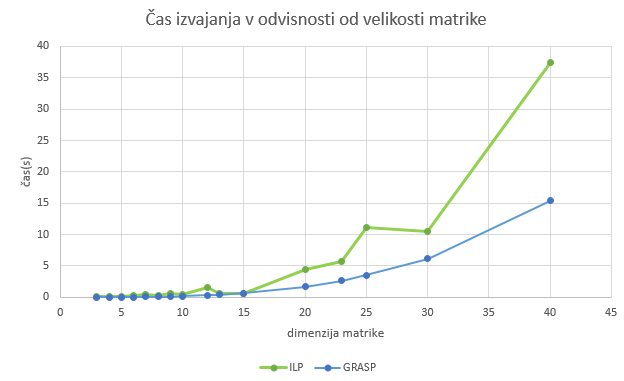
\includegraphics[scale =0.8]{casilp}
\end{figure}


\subsection{Primerjava parametra alpha} ~\\
Za primerjavo parametra alpha smo se osredoto"cili na "stiri parametre in sicer 3, 5, 10 in 15. Parameter alpha nam dolo"ca velikost RCL (restricted client list) na "zacetku algoritma GRASP v sklopu greedy randomized construction. Torej "ce je alpha enak 5, bo algoritem skonstruiral 5 za"cetnih re"sitev problema. Te bo nato local search izbolj"seval. Primerjavo smo naredili za obe metodi na 100 iteracijah, razen v zadnjem primeru na desetih, saj je bila matrika "ze prevelika. Prav tako smo naredili deset ponovitev algoritma.
"Ce si najprej ogledamo najmanj"si graf Ulysses22, lahko vidimo, da izbira parametra ne vpliva na rezultat, saj v vseh primerih vrne  znan optimalni rezultat 1273. Pri malo ve"cjem grafu Swiss42 "ze opazimo, da se rezultat oddaljuje od optimuma, ve"cji kot je alpha. Vendar pa je pri 2-opt slab"sanje o"citno hitrej"se. Pri 3-opt celo kljub slab"sem rezultatu pri alpha = 10, pri alpha = 15 vrne optimalen rezultat. Optimalen rezultat za Berlin52 je 7544, mi pa smo dobili 7616, kar je precej blizu. Se pa tu rezultat "se hitreje poslab"sa z v"canjem alpha. Spet pri 2-opt bolj kot pri 3-opt. Tudi pri St70 najbolj"si rezultat vrne 3-opt, zopet pri najmanj"sem izbranem alpha. 
Za KroA100 so rezultati "ze moCno oddaljeni od optimuma in vse bolj kot se pove"cuje alpha. 
"Ce zaklju"cimo. Opazimo da razen v primeru zelo majnih grafov



\begin{table}[h]
\begin{tabular}{lllllll}
\rowcolor[HTML]{FFCCC9} 
TSP       &      & 3 & 5 & 10 & 15 &opt \\ \hline
Ulysses22 &      &   &   &    &  &7013  \\
          & 2-opt & 7013  &  7013 & 7013   & 7013   &\\
          & 3-opt &   7013&  7013 &  7013  &  7013 & \\
Swiss42   &      &   &   &    &   &1273 \\
	& 2-opt &   1273&  1273 &   1420 &  1592 & \\
          & 3-opt &  1273 &  1273 & 1316   &  1273 & \\
Berlin52 &      &   &   &    &   &7542 \\
	 & 2-opt &  7716 & 8130 &   8629 &  10464 & \\
          & 3-opt &  7616 &  7684 &  7735  & 8705  & \\
St70      &      &   &   &    &  & 675 \\
	& 2-opt &  714 &  888 &   1211 &  1386 & \\
          & 3-opt &  684 &  754 &   878 &   & \\
KroA100   &      &   &   &    &  &21282  \\
	& 2-opt &  37162 &  54119 &   74951 &   74462& \\
          & 3-opt &   &   &    &   &
\end{tabular}
\end{table}


\subsection{Primerjava glede na število iteracij} ~\\

Pri določanju parametrov algoritma ima pomembno vlogo tudi število iteracij. Odvisnost vrednosti rešitve od števila iteracij sva preizkusili na primeru St70 (velikosti 70). Iz prejšnjega podpoglavja ugotovimo, da je za ta primer najboljši parameter alpha = 3. Zaradi velike časovne zahtevnosti metode 3opt, smo za ta primer naredili le 200 iteracij. Ugotovimo, da se vrednost rešitve izboljšuje z večanjem iteracij. Metoda 3opt je pri preizkušanju dosegla najboljši rezultat (684) že pri 100 iteracijah. Podobno rešitev pri metodi 2opt dobilo še le pri 600 iteracijah. 

\begin{figure}[h]
\caption{Odvisnost rešitve od števila iteracij}
\centering
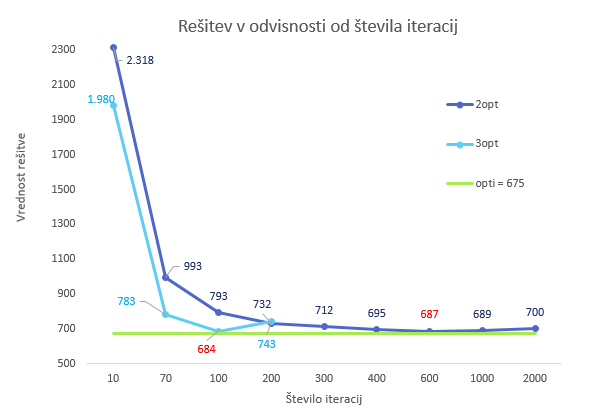
\includegraphics[scale =0.8]{resitev_iteracije}
\end{figure}

Zaradi manjše časovne zahtevnosti metode 2opt, lahko pri izvajanju GRASPA uporabimo več iteracij kot pri metodi 3opt. 
\begin{figure}[h]
\caption{Odvisnost časa izvajanja od števila iteracij}
\centering
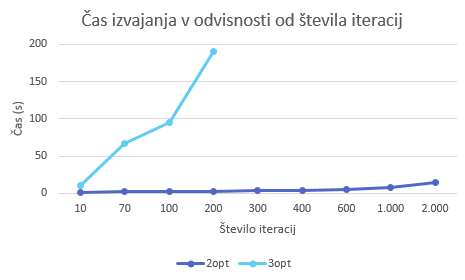
\includegraphics[scale =0.8]{cas_izvajanja}
\end{figure}

\subsection{Primerjava s skupino 7} ~\\

\begin{table}[h]
\begin{tabular}{lll}
\rowcolor[HTML]{FFCCC9} 
          & GRASP & GA \\
Ulysses22 & 7013  & 7112               \\
Berlin52  & 7616  & 8737               \\
KroA100   & 21761 & 36408             
\end{tabular}
\end{table}

\begin{figure}[h]
\caption{Najkraša pot primera berlin52 dolga 7692}
\centering
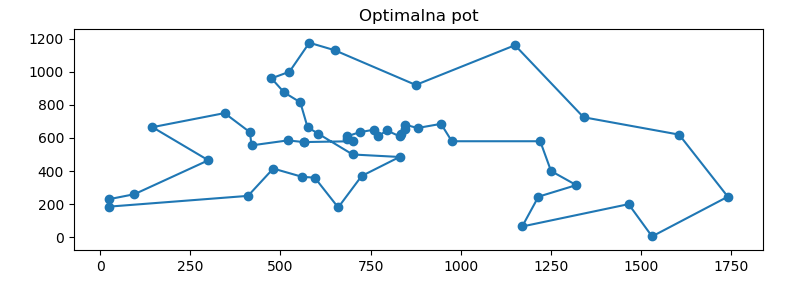
\includegraphics[scale =0.5]{berlin_7692}
\end{figure}

\begin{figure}[h]
\caption{Najkrajša pot primera ulysses22, dolga 7013}
\centering
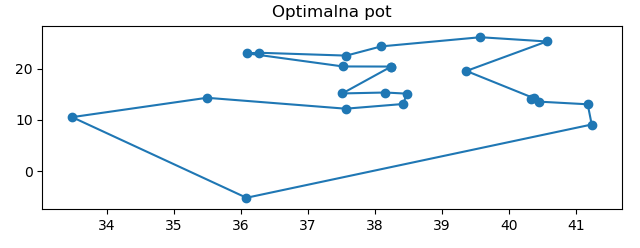
\includegraphics[scale =0.5]{ulysses22_7013}
\end{figure}

\section{Zaklju"cek}

The description of GRASP as given
above indicates that a basic GRASP does
not use the history of the search process.11
The only memory requirement is for storing the problem instance and for keeping the best so-far solution. This is one
of the reasons why GRASP is often outperformed by other metaheuristics. However, due to its simplicity, it is generally
very fast and it is able to produce quite
good solutions in a very short amount of
computation time. Furthermore, it can be
successfully integrated into other search
techniques.

\pagebreak
% seznam uporabljene literature
\begin{thebibliography}{99}

\bibitem{Wikipedia TSP}
Travelling salesman problem
\\\texttt{http://en.wikipedia.org/wiki/Travelling\_salesman\_problem}

\bibitem{}
C. Blum, A. Roli, Metaheuristics in Combinatorial Optimization: Overview and Conceptual
Comparison, online
\\\texttt{https://www.iiia.csic.es/~christian.blum/downloads/blum\_roli\_2003.pdf}

\bibitem{}
S. Luke, Essentials of Metaheuristics: a set of undergraduate lecture notes, online.
\\\texttt{https://cs.gmu.edu/~sean/book/metaheuristics/Essentials.pdf}

\bibitem{}
TSP Basics
\\\texttt{https://tsp-basics.blogspot.com/2017/03/}

\bibitem{}
R. Škrekovski, Zbornik seminarjev iz hevristik [Elektronski vir]: izbrana poglavja iz optimizacijskih metod (2010-11) / Riste Škrekovski, Vida Vukašinovič - El. knjiga. - Ljubljana: samozal. R. Škrekovski, 2012. 
\\\texttt{https://www.fmf.uni-lj.si/~skreko/Gradiva/Zbornik\_Hevristike.pdf}


\end{thebibliography}

\end{document}

